\begin{figure}[tb]
  \centering
  % 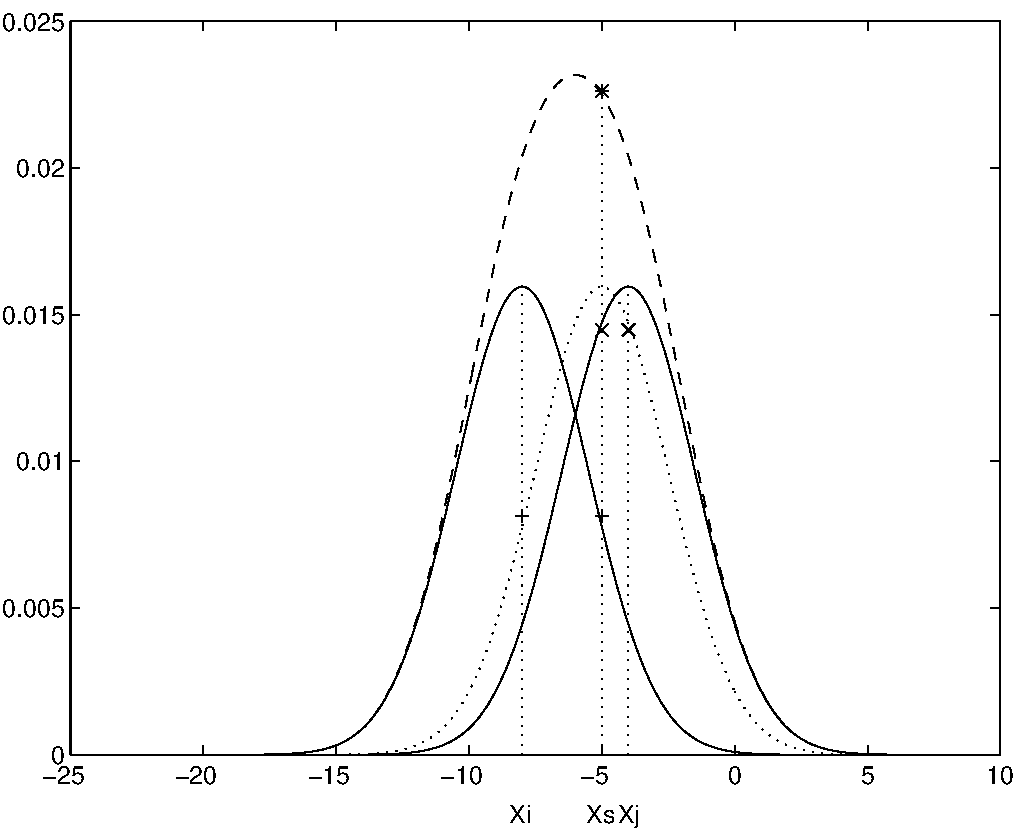
\includegraphics[height=6.5cm]{eijkel2}
  % \fbox{\rule{0pt}{0.8in} \rule{.95\linewidth}{0pt}}
  %\includesvg[inkscapelatex=false, width = 1\linewidth]{images/pipeline_frosting_largefont}
  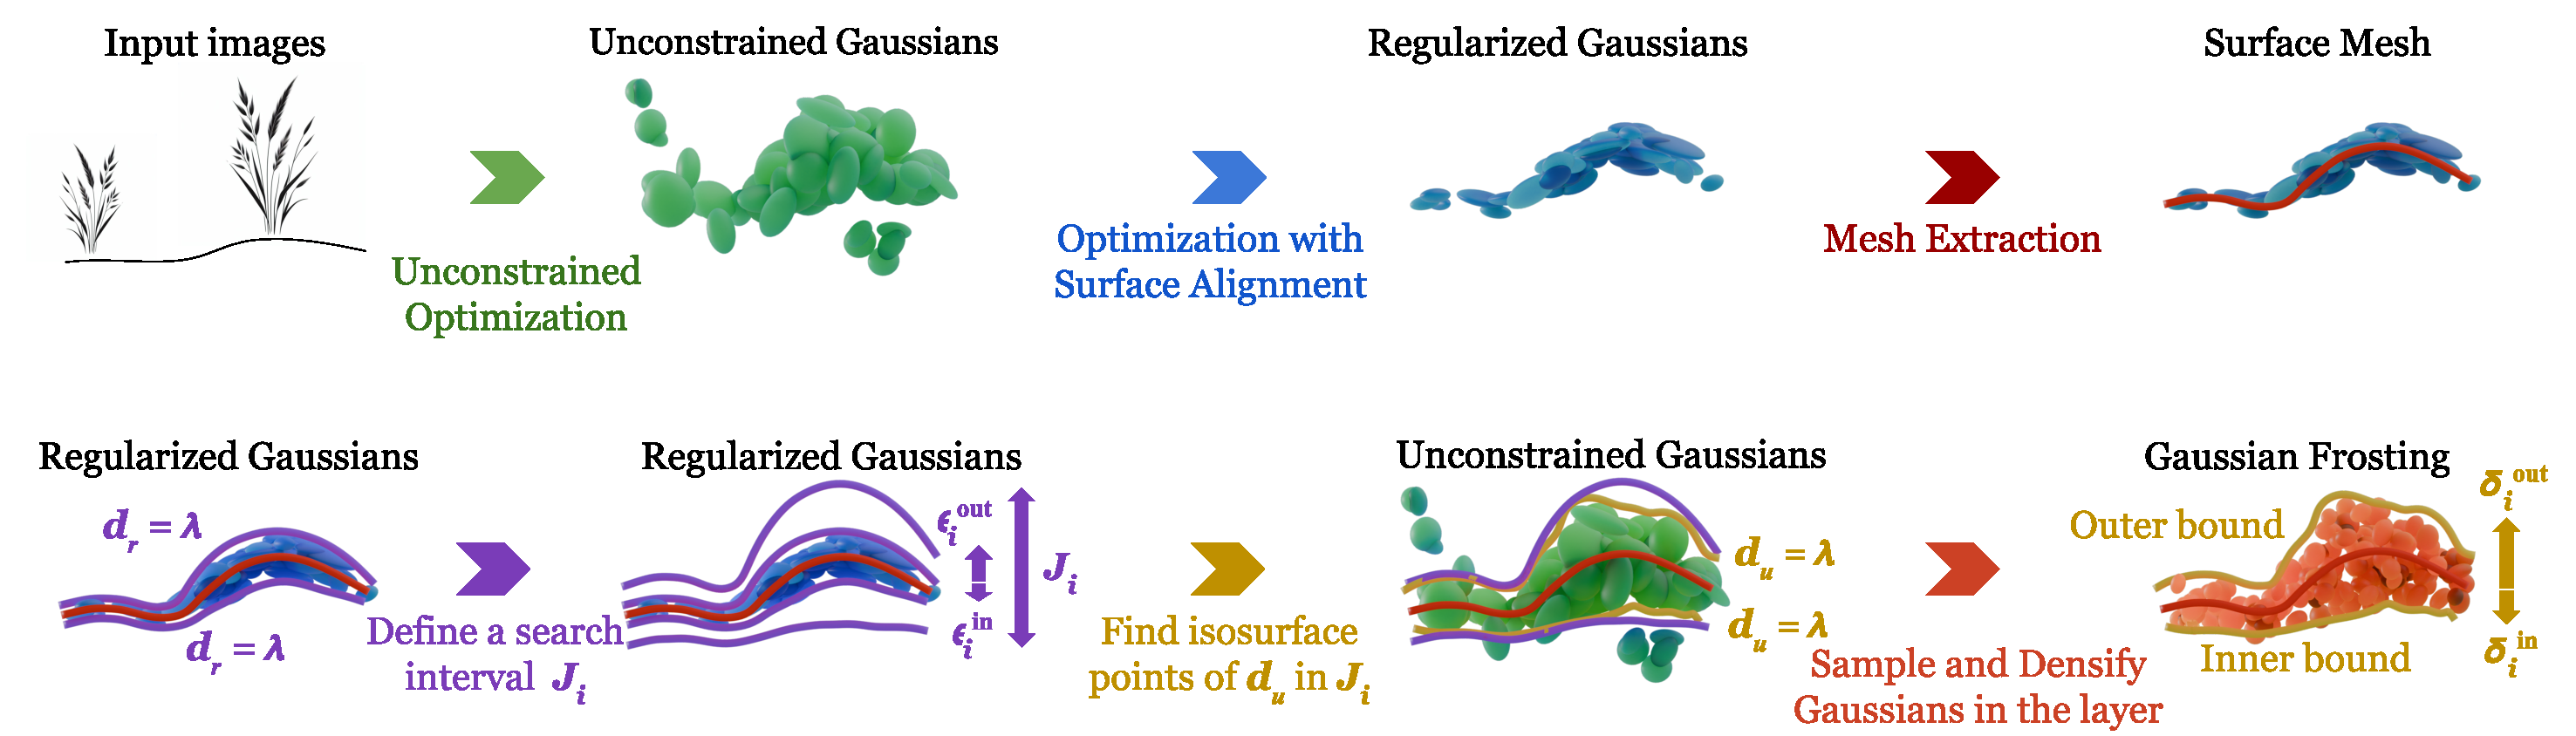
\includegraphics[width=\linewidth]{images/pipeline_frosting_largefont.pdf}
  \caption{
  \textbf{Creating a Layer of Gaussian Frosting.} To build our proposed Frosting representation, we start by optimizing a Gaussian Splatting representation using a rendering loss without any additional constraint, to let Gaussians position themselves. We refer to these Gaussians as \emph{unconstrained}. We then regularize these Gaussians to enforce their alignement with the surface, and extract a mesh that will serve as a basis for the Frosting. Next, we use the misalignment of surface-aligned Gaussians to identify areas where more volumetric rendering is needed, and we build search intervals $J_i$ around the mesh's vertices $\vec{v_i}$. Finally, we use the density function of the unconstrained Gaussians to refine the intervals, resulting in a Frosting layer. We finally sample a novel, densified set of Gaussians inside the layer.
}
  \label{fig:frosting-pipeline}
\end{figure}